\section{Einleitung}

Dieses Dokument dient als Sammlung und Dokumentation des erlernten Wissens im Rahmen der Ausbildung zum Fachinformatiker in der Fachrichtung Anwendungsentwicklung. Es ist ein umfassender Überblick über die Ausbildungsinhalte, die im Verlauf der dreijährigen Berufsausbildung bei der AXA AG und insbesondere am Georg-Simon-Ohm Berufskolleg in Köln 2023 bis 2026 vermittelt wurden. Ziel dieses Dokumentes ist es, die wesentlichen Lerninhalte zu strukturieren und so eine verständliche Übersicht über die verschiedenen Fachthemen zu bieten, die während der Ausbildung behandelt wurden.

Dieses Dokument nennt hauptsächlich theoretisches Wissen, welches in der Berufsschule vermittelt wurde und oder welches von der IHK verlangt und geprüft wird.

Für die Ausbildung ist das duale System vorgeschrieben. Diese hat sich in Deutschland ganz besonders erfolgreich erwiesen, da es den Auszubildenden ermöglicht, ihre theoretischen Kenntnisse in der Berufsschule mit praktischen Erfahrungen im Ausbildungsbetrieb zu kombinieren. Die Struktur des dualen Systems ist dabei klar gegliedert und findet auf verschiedenen Ebenen statt:

\begin{figure}[H]
    \centering
    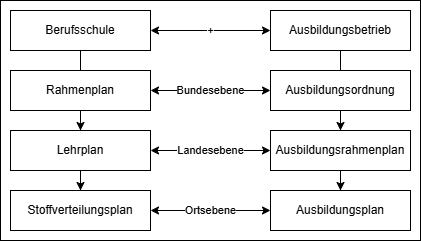
\includegraphics[width=\textwidth]{figures/dualesSystem.png}
    \caption{Duales System}
    \label{fig:dualesSystem}
\end{figure}
\FloatBarrier

Im Ausbildungsrahmenplan werden die Lernfelder wie in folgenden Kapiteln gegliedert. Darüber hinaus sieht das Land Nordrhein-Westfalen die Verknüpfung verschiedener Lernfelder in sog. Bündelungsfächer. Diese sind Gestaltung von IT-Dienstleistungen (GID), Wirtschaft- und Betriebslehre (WuB), Entwicklung vernetzter Prozesse (EvP), Cyber-Physische System (CPS), Softwaretechnologie und Datenmanagement (SuD) und IT-Grundrecht (ITG).

\begin{table}[H]
    \centering
    \begin{tabularx}{\textwidth}{|c|>{\centering\arraybackslash}X|>{\centering\arraybackslash}X|>{\centering\arraybackslash}X|>{\centering\arraybackslash}X|}
        \hline
               & GID und WuB & EvP und CPS & SuD & ITG \\
        \hline
        LF 1   & X           &             &     &     \\
        \hline
        LF 2   & X           &             &     &     \\
        \hline
        LF 3   &             & X           &     &     \\
        \hline
        LF 4   &             &             &     & X   \\
        \hline
        LF 5   &             &             & X   &     \\
        \hline
        LF 6   & X           &             &     &     \\
        \hline
        LF 7   &             & X           &     &     \\
        \hline
        LF 8   &             &             & X   &     \\
        \hline
        LF 9   &             & X           &     &     \\
        \hline
        LF 10a &             &             &     &     \\
        \hline
        LF 11a &             &             &     &     \\
        \hline
        LF 12a &             &             &     &     \\
        \hline
    \end{tabularx}
    \caption{Bündelungsfächer zu Lernfeldern}
    \label{tab:buendelfaecher}
\end{table}
\FloatBarrier